\section{Konkrete Datenmodelle}
\label{sec:concrete_model}

Die Datenmodelle welche die Informationen beinhalten aus denen der Generator ausführbaren Quellcode erzeugt, werden im folgenden Abschnitt erläutert. Dabei werden auch drei Entwurfsmuster vorgestellt welche in den Modellen Anwendung fanden, das Factory-Pattern \cref{sec:language_factory}, das Visitor-Pattern \cref{sec:language_visitor} und das Kompositum-Muster \cref{sec:language_model}.

\subsection{REST-Modell}
\label{sec:rest_model}

Zuerst muss die abstrakte Beschreibung der Spreadshirt-API von der XML-Form, bestehend aus einem \emph{WADL} (\cref{sec:wadl}) und einem oder mehreren Schemabeschreibungen (\cref{sec:document_description_formats}), in ein für den Generator verarbeitbares Format überführt werden.

Die durch die WADL-Datei beschriebene Baumstruktur muss in ein Datenmodell bestehend aus Klassen und Objekten transformiert werden.
Um effektiv mit der XML Darstellung arbeiten zu können wird diese zuerst mit einem Parser in ein DOM-Modell überführt (\cref{sec:xml_parser}) welches im Arbeitsspeicher gehalten wird und damit einen schnellen Zugriff für nachfolgende Operationen darauf erlaubt. In einem nächsten Schritt wird das DOM-Modell, welches noch viele XML spezifische Informationen enthält, auf die wesentlichen API beschreibenden Merkmale reduziert. Im Gegensatz zu der in \cref{fig:wadlstructure} veranschaulichten Webanwendungsbeschreibung werden Referenzen durch deren Definition im Modell ersetzt.

\begin{figure}[tb]
    \begin{center}
        \includegraphics[width=0.5\textwidth]{resources/restmodel}
    \end{center}
    \caption{UML Klassendiagramm des REST-Modells}
    \label{fig:restmodel}
\end{figure}

Wurzelelement des Modells (siehe \cref{fig:restmodel}) ist die \textbf{Application}, über diese Klasse kann auf alle \emph{Ressourcen}-Klassen zugegriffen werden. Es enthält außerdem den Basisbezeichner der API bspw. \texttt{http://api.spreadshirt.net/api/v1/}. 

Eine \textbf{Ressource}-Klasse enthält eine Menge von \emph{Method}-Objekten, sowie einen Ressourcenbezeichner, dieser ist relativ zum Basisbezeichner des Wurzelelements. Die Ressourcenbezeichner können \emph{Template-Parameter} enthalten, diese werden bei einer Anfrage durch einen konkreten Wert ersetzt. Beispielweise enthält der Bezeichner für die Ressource eines bestimmten Users den Template-Parameter \{userid\}, vollständiger Ressourcenbezeichner \texttt{users/\{userid\}}. Ressourcenbezeichner werden durch die Klasse \textbf{SplitPath} repräsentiert. 

Jede \textbf{Method}-Klasse enthält ein \emph{Request} und ein \emph{Response} Objekt. Sie enthalten die nötigen Informationen für eine Anfrage auf eine Ressource, bzw. den Aufbau der Antwortnachricht.

Eine \textbf{Request}-Klasse enthält eine Liste von Query-Parametern sowie ein \emph{Representation} und \emph{Response} Objekt.

\textbf{Parameter} enthält Angaben zum \emph{Style}, Typ, Vorgabewert und ob dessen Angabe \enquote{required}, also notwendig ist. Die Angabe des Typs ist eine Referenz auf einen Typ aus einer XML-Schemabeschreibung. Der \emph{Style} gibt an wie der Parameter übermittelt wird, als Teil der Query \texttt{\ldots{}?mediaType=xml}, \emph{Key-Value Pair} des HTTP-Header oder als \emph{Template-Parameter} des Ressourcenbezeichners. 

Die Klasse \textbf{Response} enthält eine Menge von \emph{Representations}, sowie eine Liste von Parametern. Die \emph{Representations} enthalten die Beschreibung der Daten die bei einer erfolgreichen Anfrage an die Ressource zurückgesendet werden, sowie die der Fehlermeldung die der Client anderenfalls erhält. Zwischen einer Fehlermeldung und einer Antwort auf eine erfolgreiche Anfrage kann anhand des Werts des HTTP-Statuscodes unterschieden werden. Erfolgreiche Antworten liefern meist einen Statuscode 200 \textbf{OK} oder 201 \textbf{Created} zurück. Die Response Parameter geben Einträge im HTTP-Header an, welche für den Client nützliche Informationen enthalten. Legt der Client z.B. via POST auf der Ressource \texttt{sessions} eine neue API-Session an, so enthält das Feld \texttt{Location} des HTTP-Headers der Serverantwort, die URL auf die Ressource der angelegten Session.

Die \textbf{Representation}-Klasse dient zur Beschreibung der Daten welche entweder zur API gesendet oder von dieser empfangen werden, sie besteht aus einer Angabe des \emph{media-type}, des HTTP-Statuscodes und eine Referenz auf die Definition des Datentyps. Das \emph{Representation}-Objekt eines Request einer PUT- oder POST-Methode charakterisiert zum Beispiel den Aufbau der Daten welche der Ressource übermittelt werden, üblicherweise im HTTP-Body. Die Charakterisierung erfolgt dabei in Form einer Referenz auf einen Typ aus einer Schemabeschreibung sowie der Angabe des \emph{media-type}. Beispielsweise enthält das \emph{Representation}-Objekt der PUT-Methode auf Ressource \texttt{users/\{userId\}/designs/\{designId\}} den media-type \texttt{application/xml} und eine Referenz auf den Typ \texttt{sns:design}. 

Referenzen auf Typdeklaration aus einer Schemabeschreibung werden nachfolgend im Modell durch die konkrete Deklaration des Typs aus der XML-Schemabeschreibung ersetzt, siehe \cref{sec:application_model}. 

Ein Objekt der \textbf{Doc}-Klasse enthält einen Titel und eine Kurzbeschreibung des zugehörigen Elements.
Der Generator erzeugt daraus Quellcodekommentare für die Dokumentation der Bibliothek.

\subsection{Schema-Modell}
\label{sec:schema_model}

Wurzel des Schemadatenmodells ist die Klasse \textbf{Schema}. Ein Schema kann Objekte vom Typ \emph{Complex-} und \emph{SimpleType} sowie \emph{Attribute} und \emph{Element} enthalten.

XSD-Dateien (siehe \cref{sec:xsd}) erlauben das importieren anderer Schemadefinitionen, die Klasse \textbf{Import} ermöglicht dies im Schemamodell. Ein Objekt der Klasse besitzt das zu importierende Schema sowie dessen Namespace und einen Verweis auf die XSD-Datei.

Die \textbf{ComplexType}-Klasse repräsentiert die gleichnamigen strukturierten Typen aus der Schemadefinition. 

Objekte der Klasse \textbf{Element} besitzen einen Bezeichner, sowie einen Complex- oder SimpleType und optional eine Angabe der Auftrittshäufigkeit.
... ElementParameter dient zur Vereinfachung der konstruktion solcher objekte...

Durch die Klasse \textbf{Namespace} werden der Präfix und der Bezeichner des \emph{Namensraums} eines Typs aus dem Schema gekapselt. Ein Namespace im Schemamodell ist folgendermaßen aufgebaut: 
\[  
    \underbrace{tns}_{\small \text{Präfix}}:\underbrace{http://api.spreadshirt.net}_{\small \text{Bezeichner des Namensraumes}}
\]

\begin{figure}[tb]
    \begin{center}
        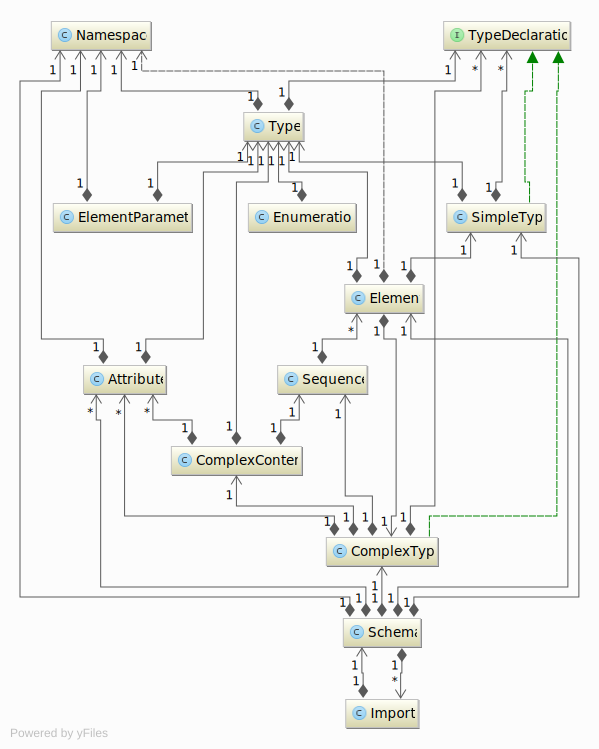
\includegraphics[width=0.6\textwidth]{resources/typemodel}
    \end{center}
    \caption{UML Klassendiagramm des Schemadatenmodells}
    \label{fig:schema_model}
\end{figure}

\subsection{Applikationsmodell}
\label{sec:application_model}

\subsection{Sprachenmodell}
\label{sec:language_model}

\begin{figure}[tb]
    \begin{center}
        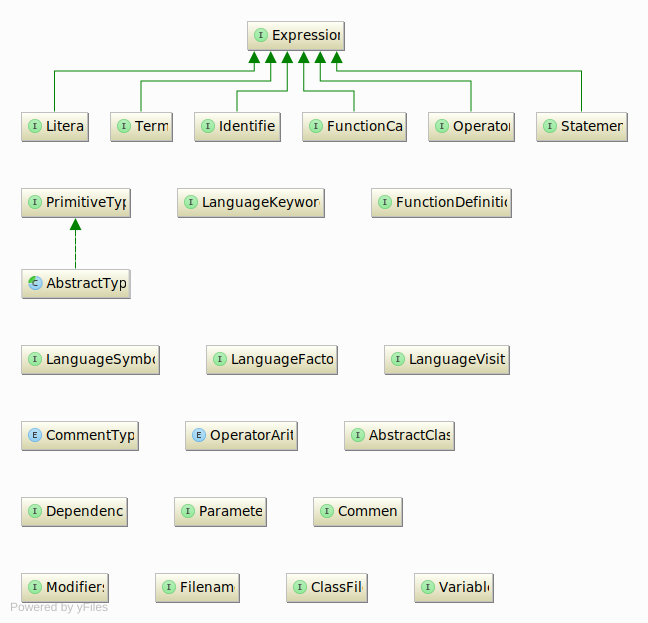
\includegraphics[width=0.6\textwidth]{resources/languagemodel}
    \end{center}
    \caption{UML Klassendiagramm des Zielsprachenmodells}
    \label{fig:language_model}
\end{figure}

\begin{lstlisting}[
        basicstyle=\footnotesize,
        stringstyle=\ttfamily,
        identifierstyle=\color{black},
        stringstyle=\color{black},
        keywordstyle=\color{black},
        numbers=none,
        caption=EBNF des Expression-Typs aus dem Zielsprachenmodell
    ]
Expression 
    = Literal 
    | Identifier
    | Term
    | FunctionCall
    | Operator
    | Statement
    | Condition ;
Term 
    = [Expression] Operator Expression 
    | Expression ;
FunctionCall = {Parameter} Name ReturnType ;
Operator = Symbol ;
Statement 
    = IdentifierTerm 
    | Term ;
Condition = Term{Statement} ;
Literal = PrimitiveType ;
Identifier = Name ;
PrimitiveType = Prefix Value Postfix ;
Prefix = String ;
Postfix = String ;
Value = String ;
Name = String ;
ReturnType = String ;
Symbol = String ;
String = '"' {UTF-8} '"'

\end{lstlisting}

\subsection{Language Visitor}
\label{sec:language_visitor}

Kapitel gehört eher zu Generator

\subsection{PHP-Zielsprachenmodell}
\label{sec:php_target_language_model}

% Sprachschnittstelle!
\subsection{Language Factory}
\label{sec:language_factory}

Um eine Zielsprachenunabhänhigkeit zu erreichen, wird dem Generator bei der Erzeugung eine \enquote{Language Factory} übergeben. Der Generator erzeugt Sprachelemente nur über diese Factory. Ein Aufruf einer Factorymethode gibt ein Element der vom Typ der Sprache zurück, der Generator kennt aber nur den Interface-Typ. Für ihn ist die konkrete Implementierung somit transparent.
